%!TEX program = xelatex
%!BIB program = bibtex

\documentclass[en,black,10pt,normal]{elegantnote}
\usepackage{float}
\usepackage{hyperref}

\newcommand{\upcite}[1]{\textsuperscript{\textsuperscript{\cite{#1}}}}

\title{Practical 4 Sequence alignment}
\author{WenYuan Jiang\\ID: 1951510}
\institute{School of Life Science, Tongji University}
%\version{1.00}
\date{April 17, 2021}
\AtBeginEnvironment{lstlisting}{\linespread{0.75}\selectfont}

\begin{document}

\maketitle

\section{Align the two pairs of sequences in supplement or your interested sequences (both nucleotide and protein sequences) by using local alignment and global alignment tools and compare the results.}

\subsection{Homo sapiens (human) alpha globin vs. Mus musculus (house mouse) alpha-globin}

Two sequences used in Pairwise Sequence Alignment is collected from the supplement on canvas,
which is downloaded from The European Nucleotide Archive (ENA).

The url for downloading the data is \url{https://www.ebi.ac.uk/ena/browser/view/CAA23748} and \url{https://www.ebi.ac.uk/ena/browser/view/CAA24095}.

Since the two sequences are from mammals, and they are orthologs, it is reasonable that 
they share a high similarity in their sequence. 
This orthology can be helpful for the choice of parameters.


\subsubsection{Global alignment}
The global alignment tool used in the analysis is \texttt{EMBOSS Needle}. \upcite{likic2008needleman}
A set of typical parameters used in this global alignment is shown below.
\begin{table}[H]
    \caption{Parameters of \texttt{Needle}}
    \centering
    \begin{tabular}{cc}
        \toprule
        Key&Value\\
        \midrule
        datafile&EDNAFULL\\
        gapopen&10.0\\
        gapextend&0.5\\
        endopen&10.0\\
        endextend&0.5\\
        \bottomrule
    \end{tabular}
\end{table}

A typical summary of the output is listed below.

\begin{table}[H]
    \caption{Results of \texttt{Needle}}
    \centering
    \begin{tabular}{cc}
        \toprule
        Key&Value\\
        \midrule
        Length&142\\
        Identity&350/433 (80.8\%)\\
        Similarity&350/433 (80.8\%)\\
        Gaps&8/433 ( 1.8\%)\\
        Score&1398.5\\
        \bottomrule
    \end{tabular}
\end{table}

An example of detailed alignment and the full datafile is provided in the Supplementary materials section.

We changed the scoring matrix for the program, and the results is shown in the figure below.

\begin{figure}[H]
    \centering
    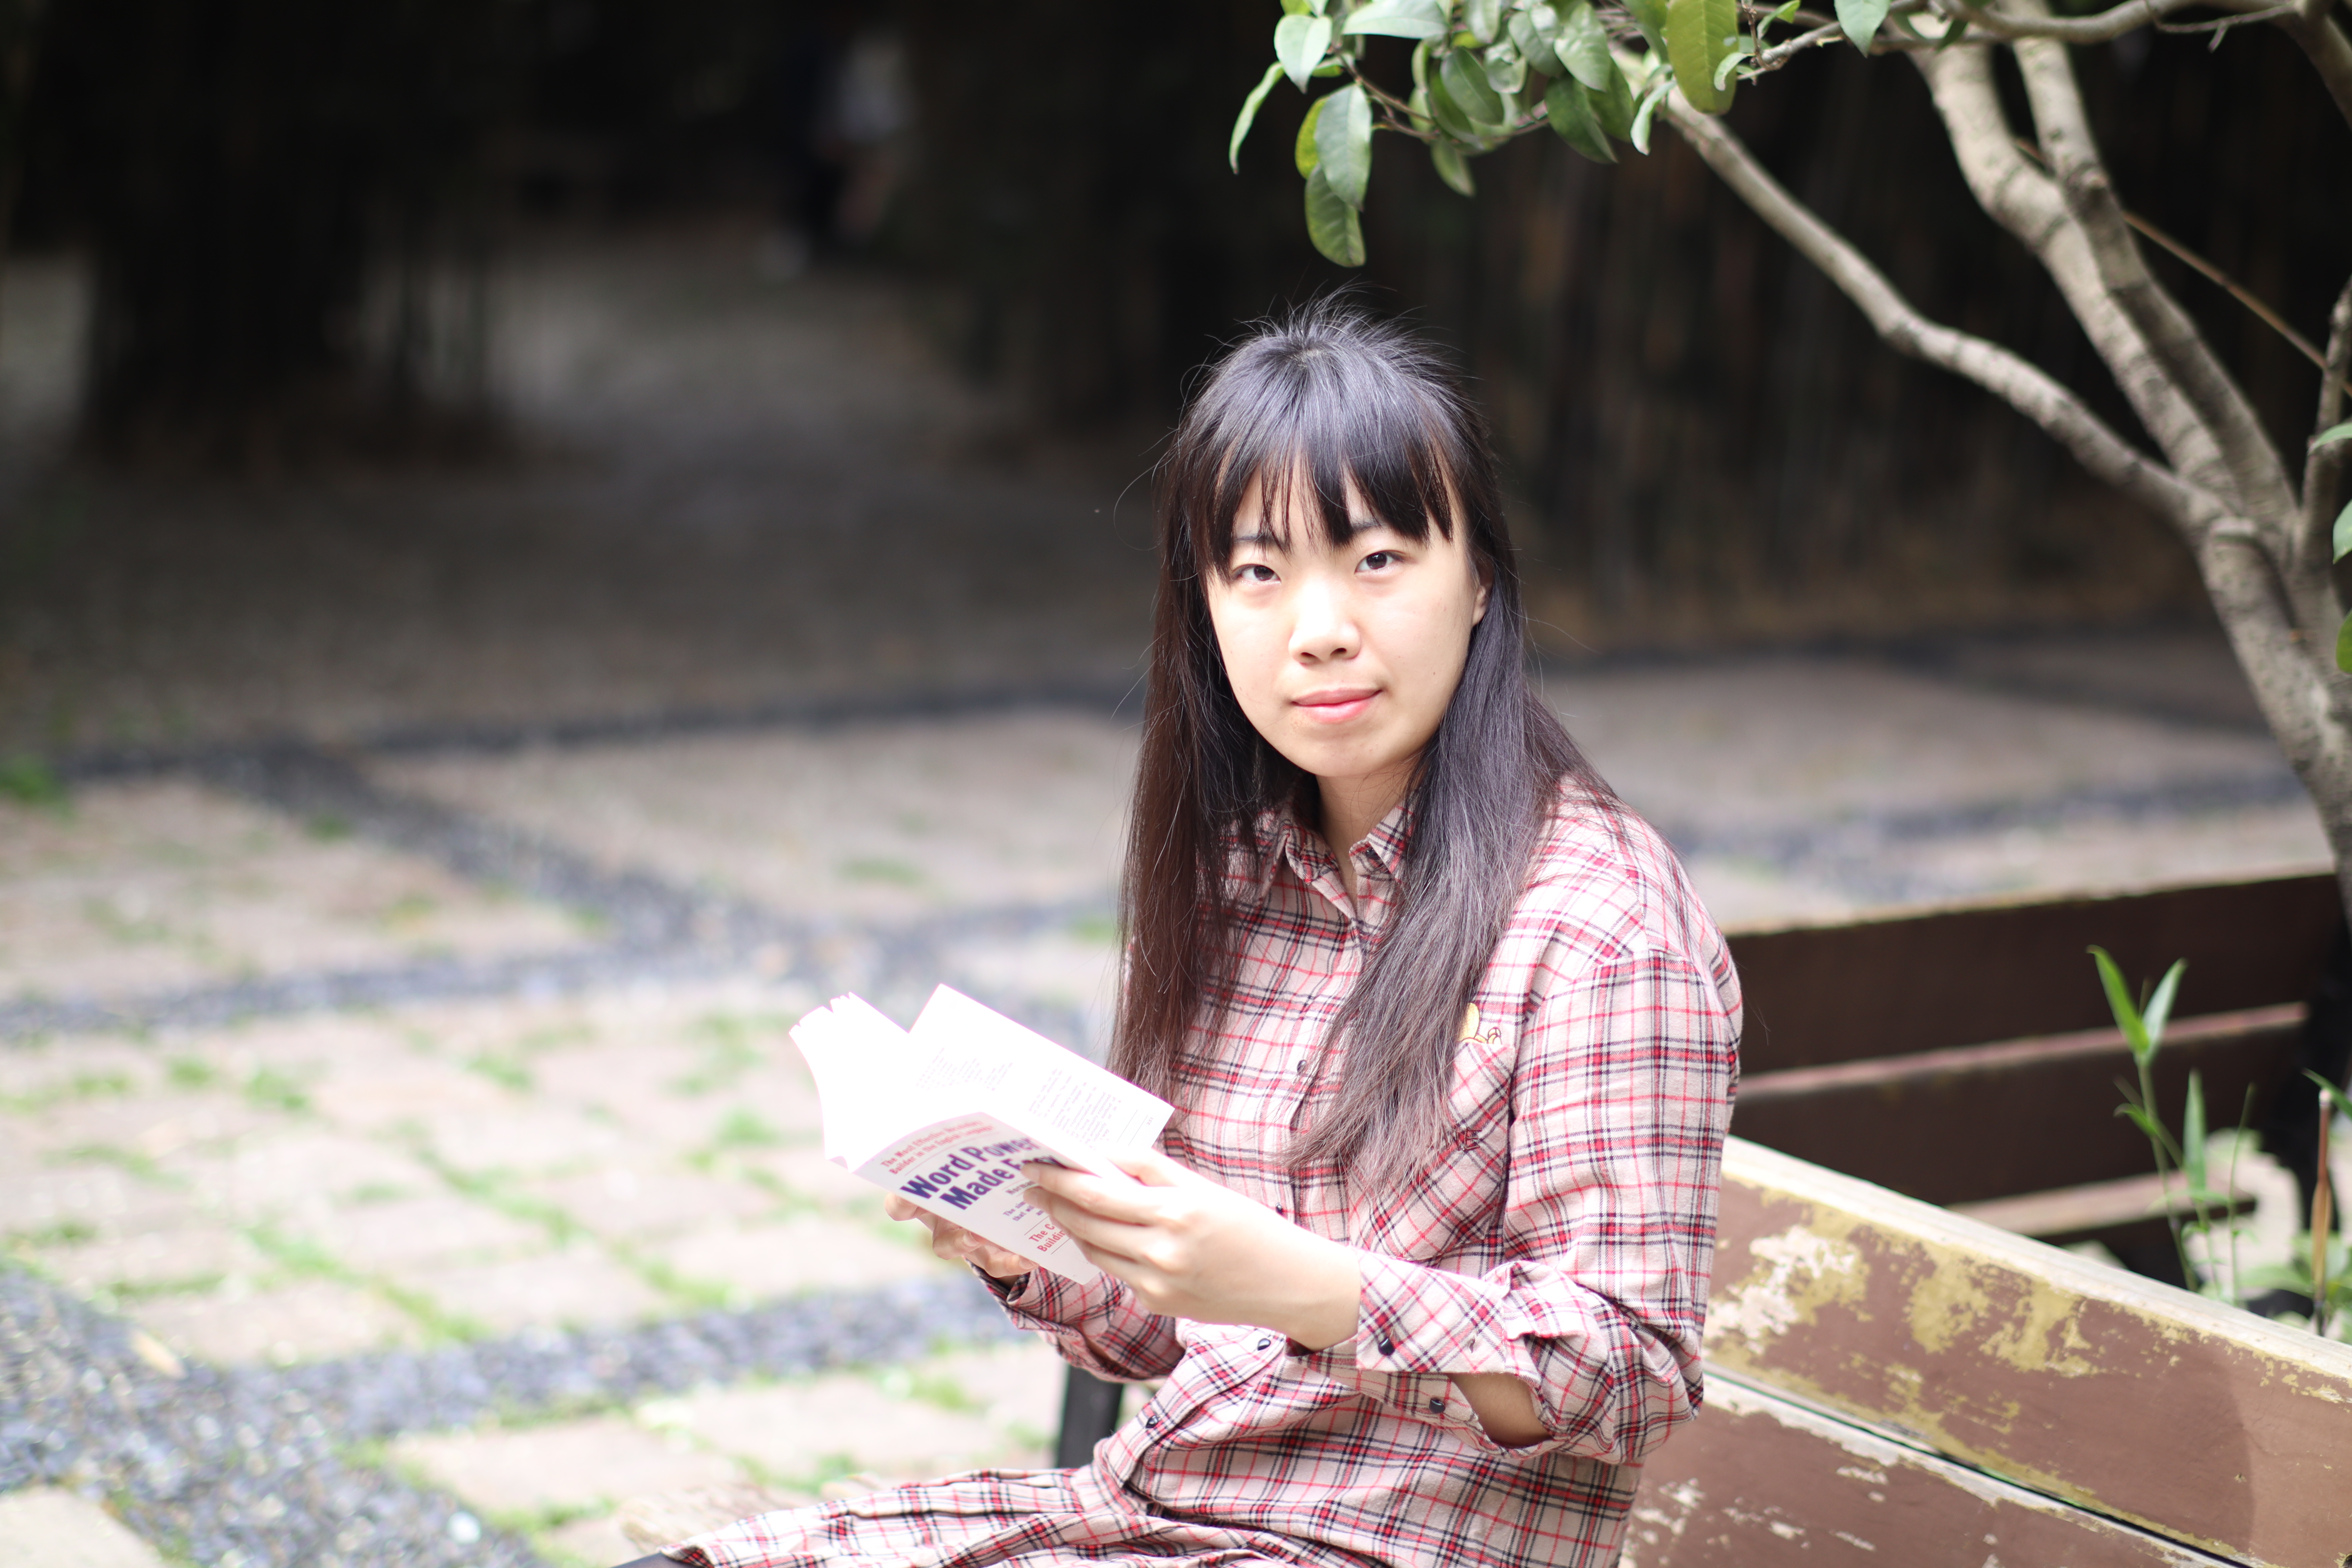
\includegraphics[width=1\textwidth]{F1}
    \caption{Alignments produced by \texttt{Needle} using different scoring matrix}
    \label{F1}
\end{figure}

As is shown in Fig.1 above, different scoring matrix have some impact on the alignment.
However, since the two sequences are highly similar, the results do not vary much.

Next, we changed the penalty for Gapopen and Gapextend for the alignment, 
and \texttt{Needle} produced different results as in Fig.2.

\begin{figure}[H]
    \centering
    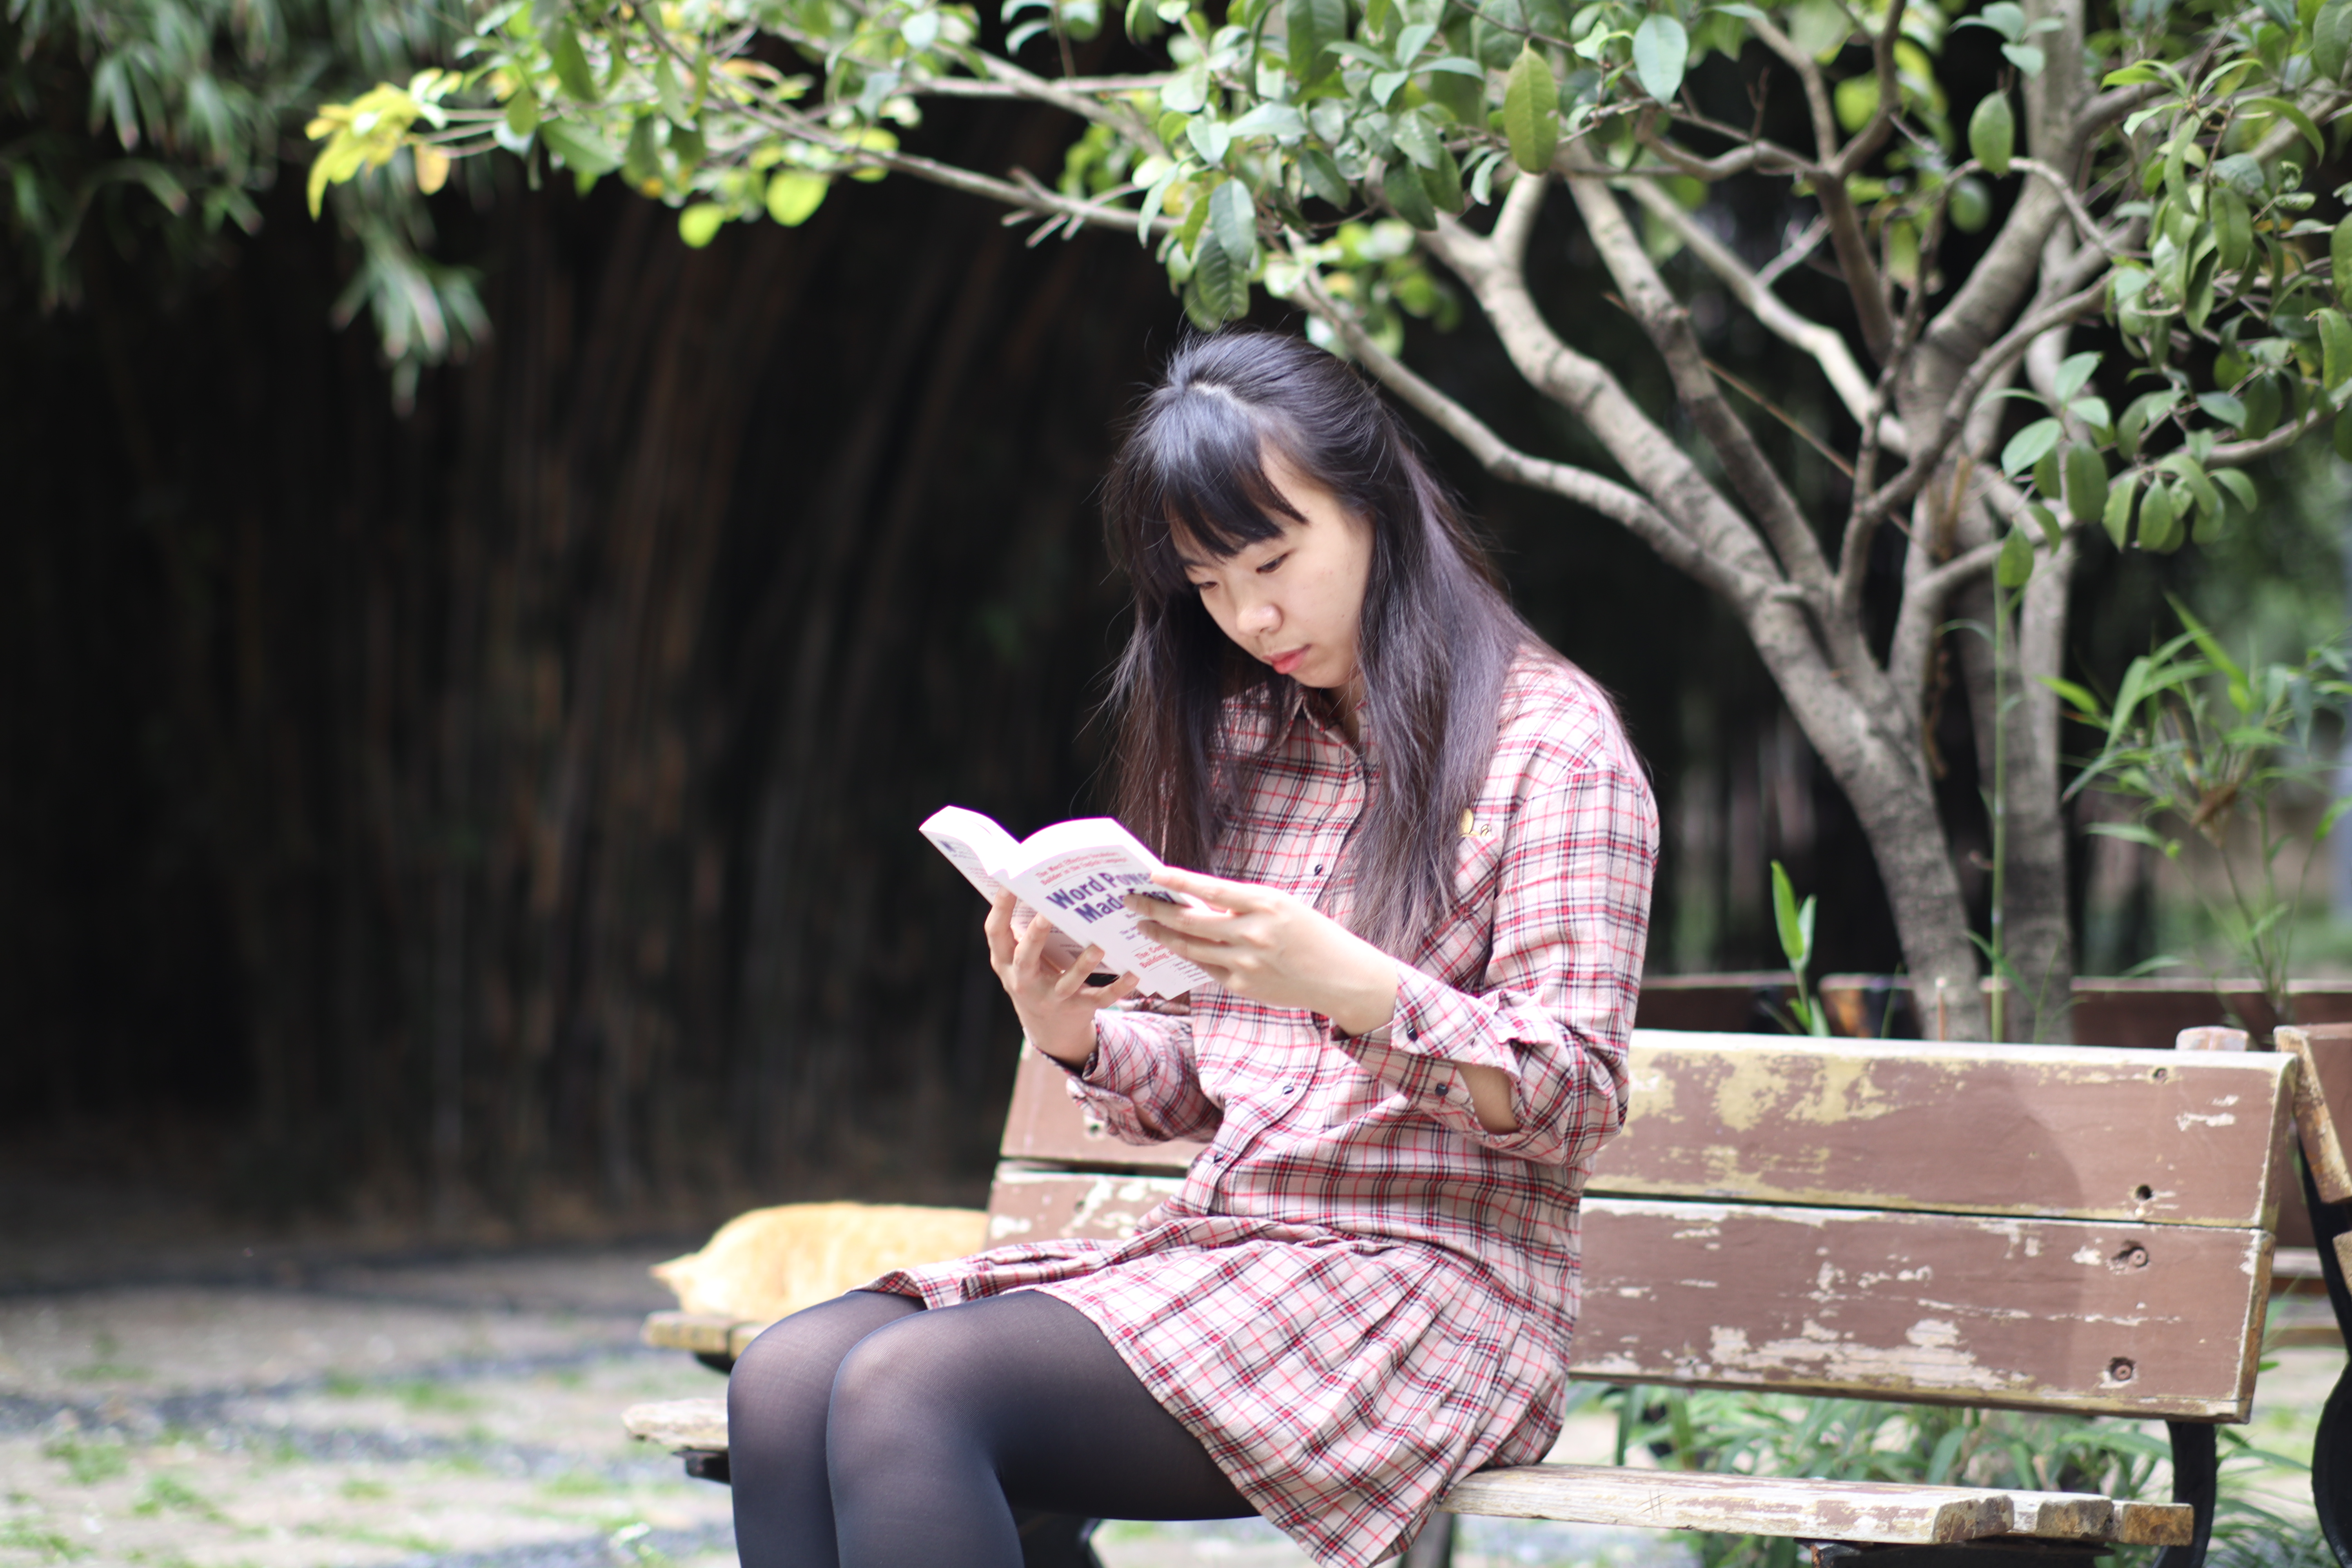
\includegraphics[width=1\textwidth]{F3}
    \caption{Alignments produced by \texttt{Needle} using Gapopen/Gapextend ratio}
    \label{F2}
\end{figure}

We expected that the Gapopen/Gapextend ratio can change the result given by the program, 
and when the ratio gets larger, \texttt{Needle} favours less and longer gaps than
more short gaps. Since the sequences here is highly similar, overall the alignment changed little
under different parameters.

\subsubsection{Local alignment}


The local alignment tool used in the analysis is \texttt{EMBOSS Water}\upcite{smith1981comparison}, 
which is similar to the \texttt{EMBOSS Needle} in input and output format.

Since the sequences we used is highly homologous, Local alignment produced nearly the same results as the global alignment.
The results are shown in the figures below, with different Gapopen/Gapextend ratio, and only when the Gapopen/Gapextend ratio
is small, the results have more gaps than that of global alignment.

\begin{figure}[H]
    \centering
    \includegraphics[width=1\textwidth]{Fig3}
    \caption{Alignments produced by \texttt{Water} using Gapopen/Gapextend ratio}
    \label{Fig3}
\end{figure}



\subsection{Homo sapiens (human) Hemoglobin subunit alpha vs. Mus musculus (house mouse) Hemoglobin subunit alpha}

The local alignment tool used in the analysis is \texttt{EMBOSS Water}. 
Typical parameters used in this loacl alignment is shown below.

\subsubsection{Global alignment}
\begin{table}[H]
    \caption{Parameters of \texttt{Needle}}
    \centering
    \begin{tabular}{cc}
        \toprule
        Key&Value\\
        \midrule
        datafile&EDNAFULL\\
        gapopen&10.0\\
        gapextend&0.5\\
        endopen&10.0\\
        endextend&0.5\\
        \bottomrule
    \end{tabular}
\end{table}

An example of detailed alignment and the full datafile is provided in the Supplementary materials section.

We changed the scoring matrix for the program, and the results is shown in the figure below.

\begin{figure}[H]
    \centering
    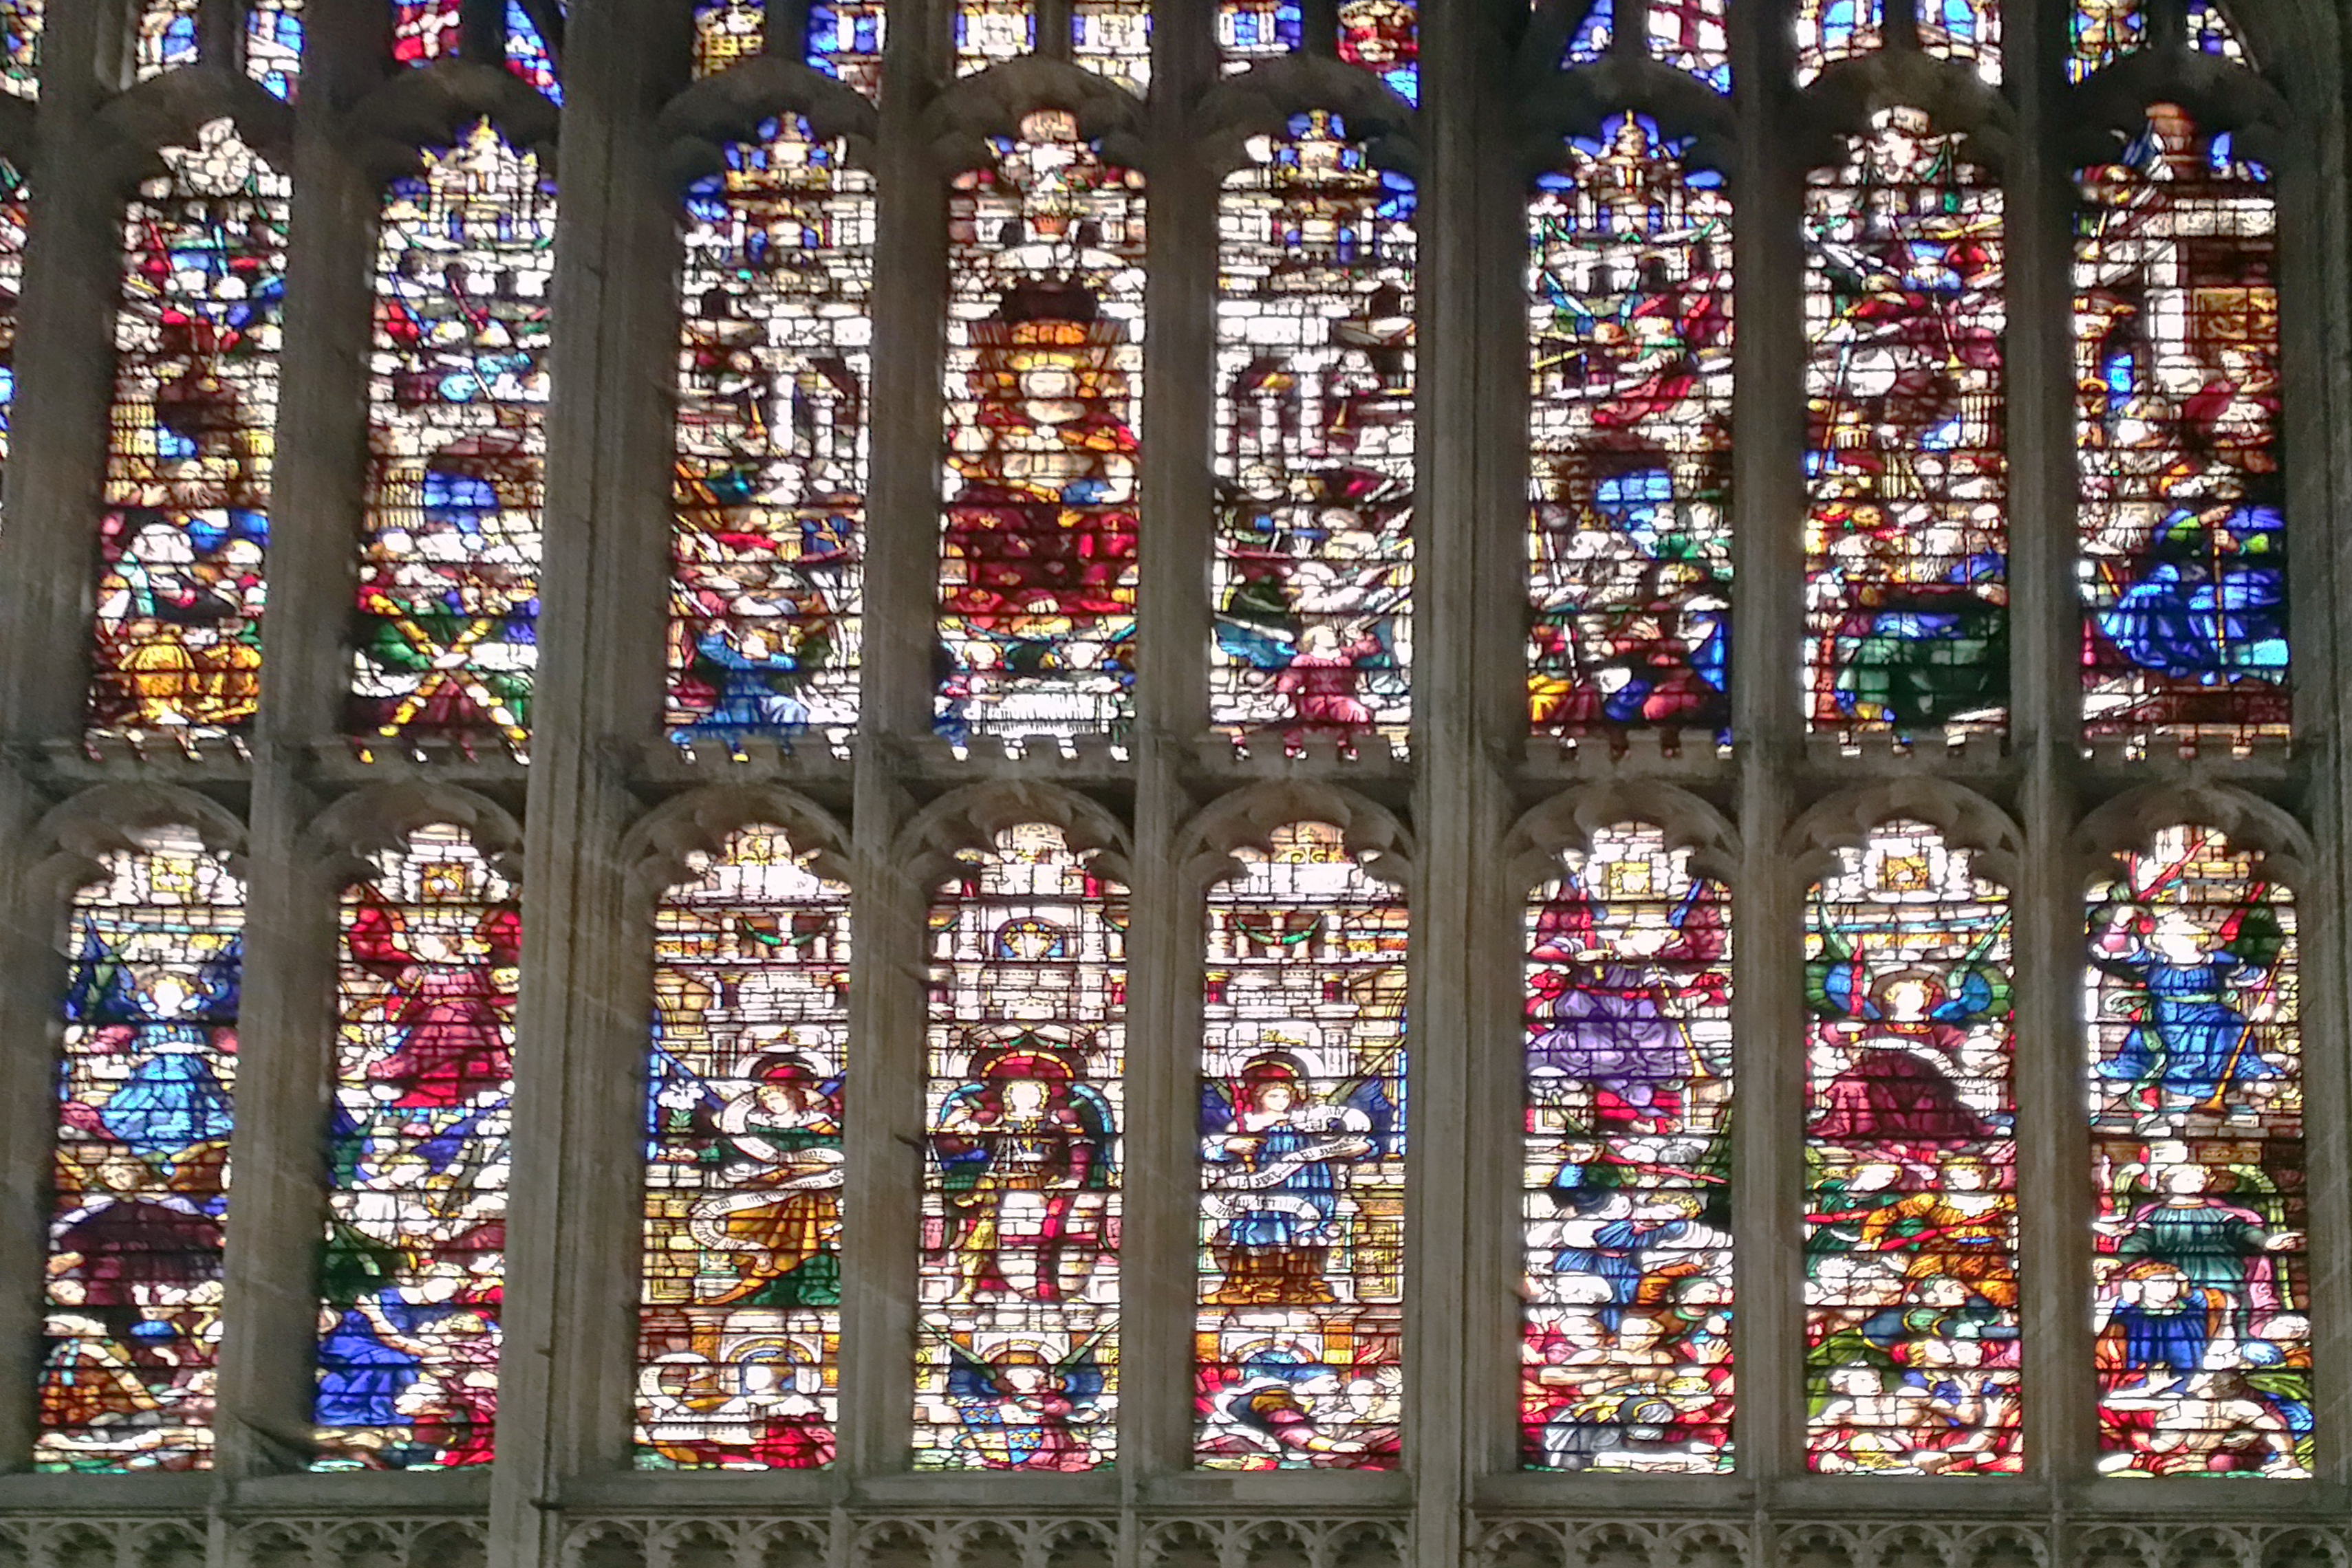
\includegraphics[width=1\textwidth]{F2}
    \caption{Alignments produced by \texttt{Needle} using different scoring matrix}
    \label{F3}
\end{figure}

As is shown in Fig.3 above, different scoring matrix have some impact on the alignment.
We had expected that BLOSUM80 will give out more reasonable results than BLOSUM30
when it comes to similar sequences, and PAM30 will give more reasonable results than PAM100.
However, since the two sequences are highly similar, the results is almost the same.

Next, we changed the penalty for Gapopen and Gapextend for the alignment, 
and \texttt{Needle} produced different results as in Fig.2.

\begin{figure}[H]
    \centering
    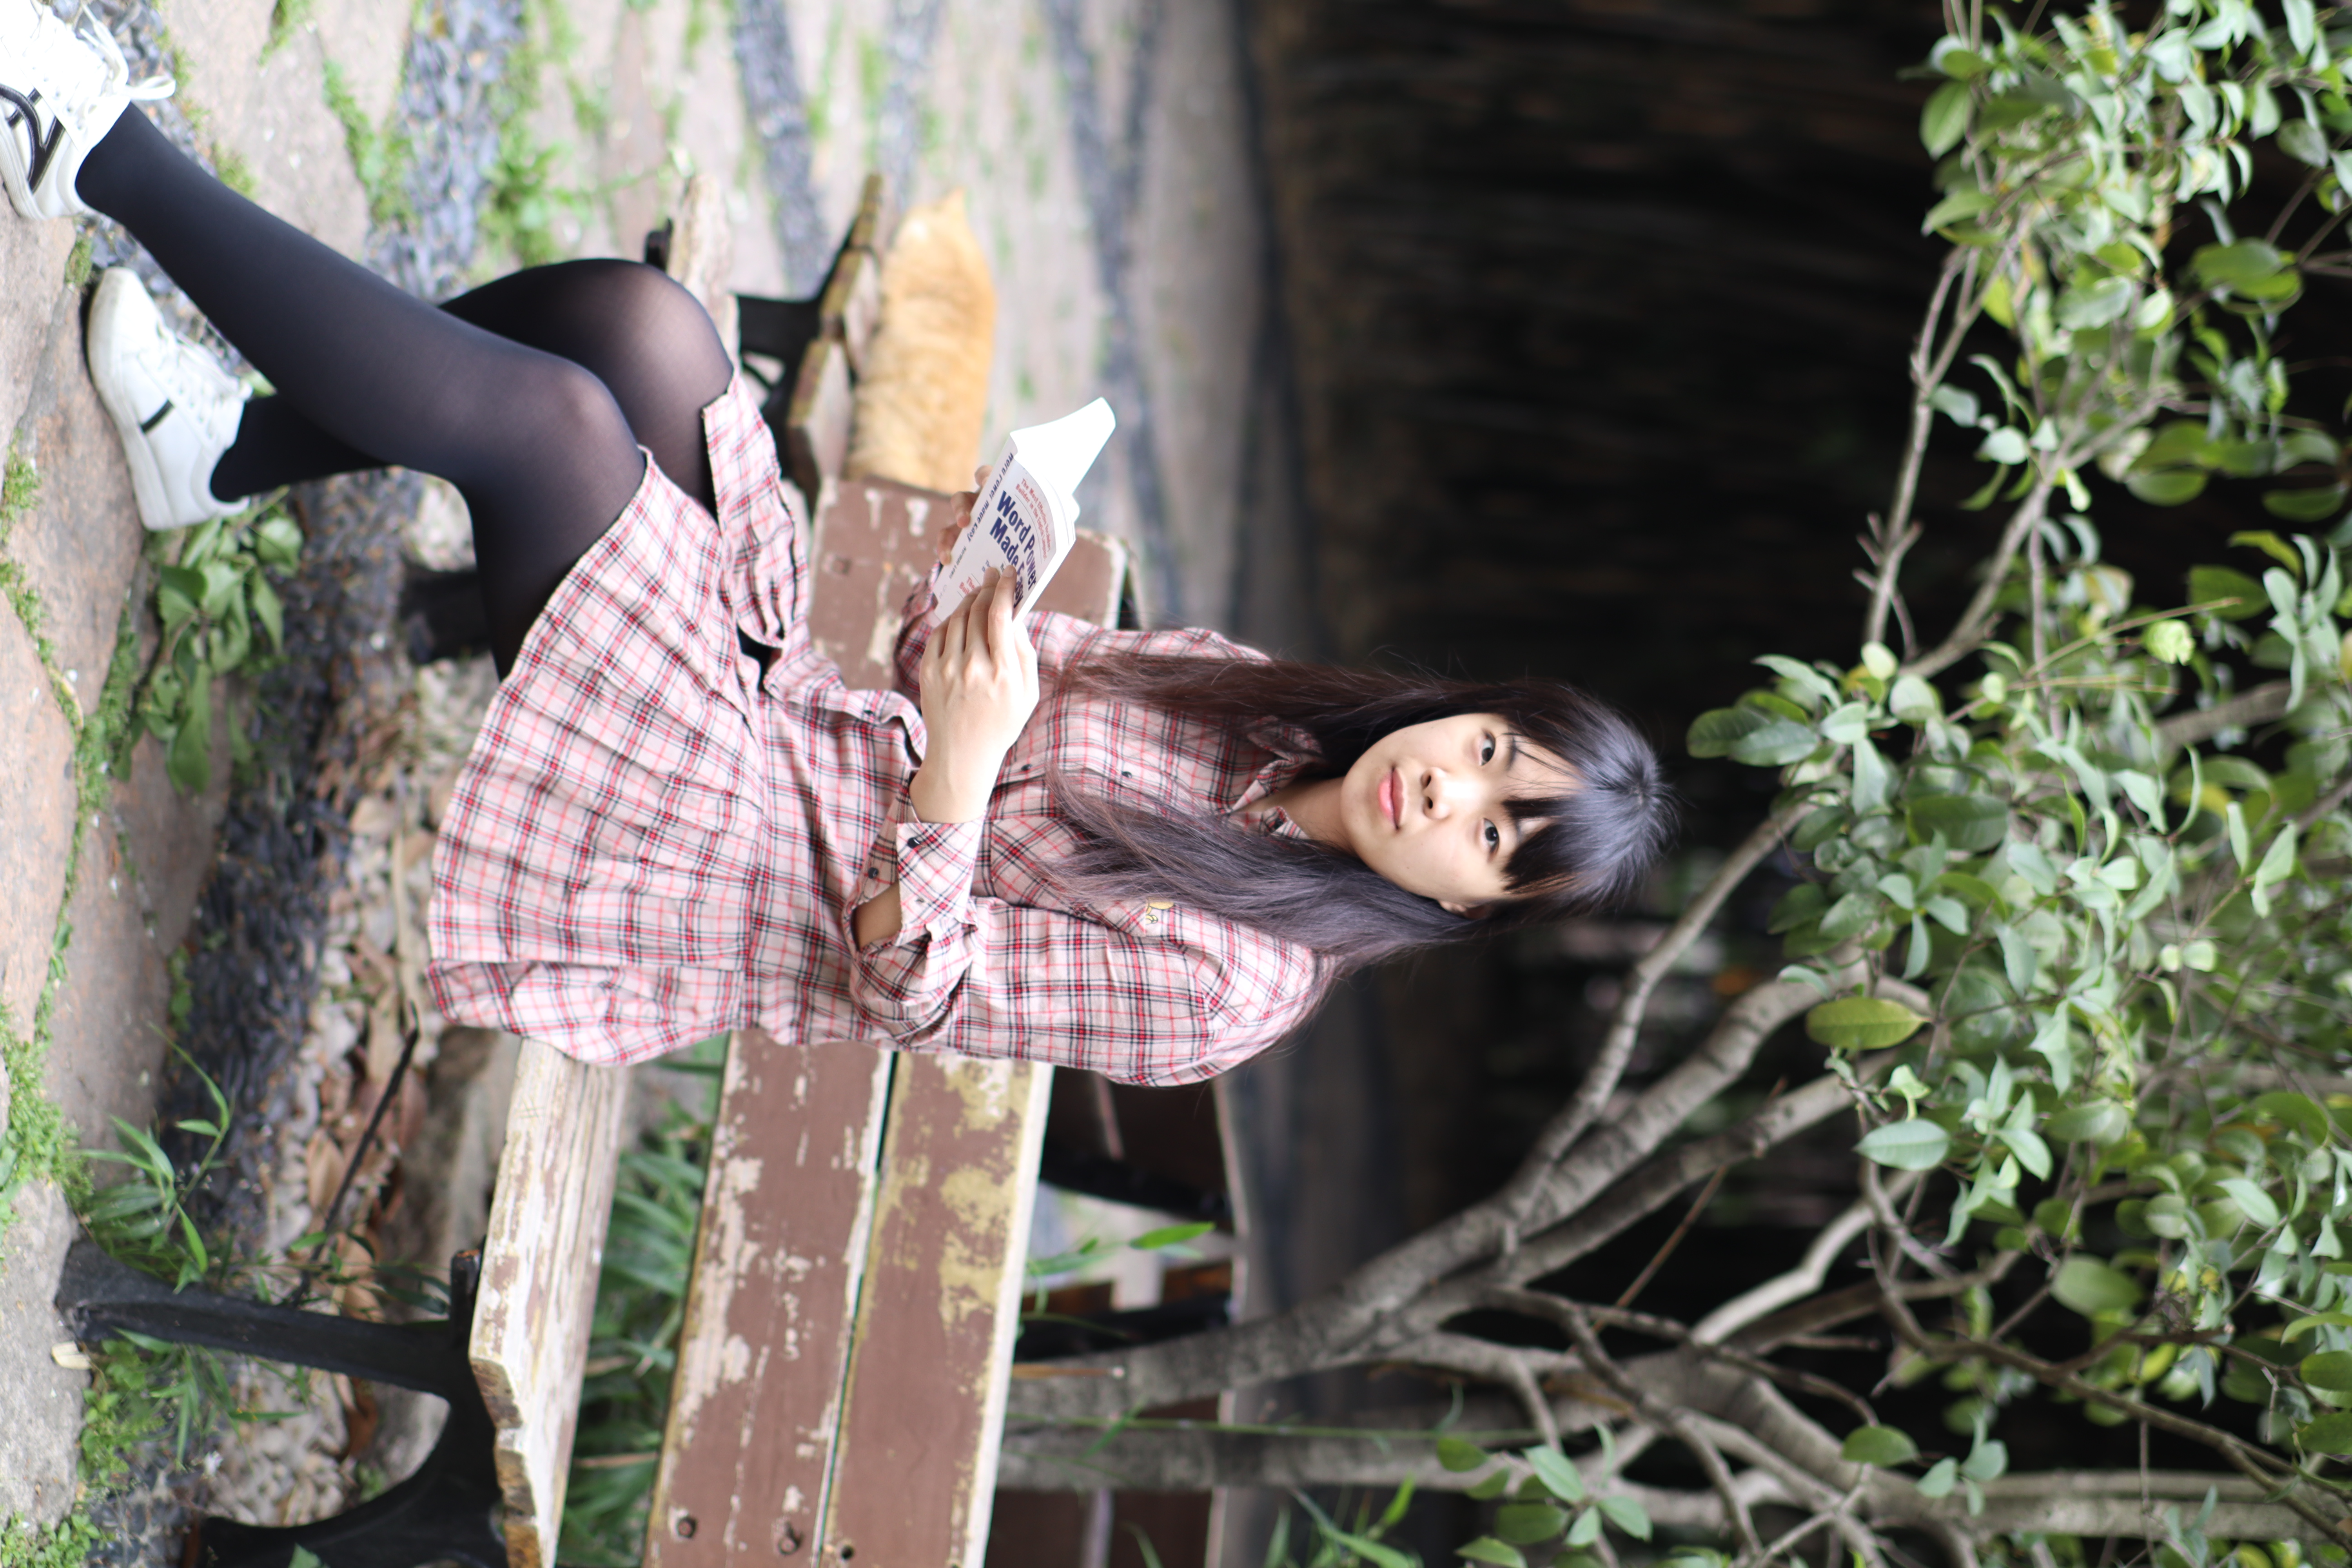
\includegraphics[width=1\textwidth]{F4}
    \caption{Alignments produced by \texttt{Needle} using Gapopen/Gapextend ratio}
    \label{F4}
\end{figure}

Since the sequences here is highly similar, overall the alignment changed little
under different parameters. Note that the Gapopen/Gapextend ratio can change the result given by the program, 
and when the ratio gets larger, \texttt{Needle} favours less and longer gaps than
more short gaps.


\subsubsection{Local alignment}

The local alignment tool used in the analysis is \texttt{EMBOSS Water}, 
which is similar to the \texttt{EMBOSS Needle} in input and output format.

Since the sequences we used is highly homologous, Local alignment produced nearly the same results as the global alignment.
The results are shown in the figures below, with different Gapopen/Gapextend ratio, and only when the Gapopen/Gapextend ratio
is small, the results have more gaps than that of global alignment.

\begin{figure}[H]
    \centering
    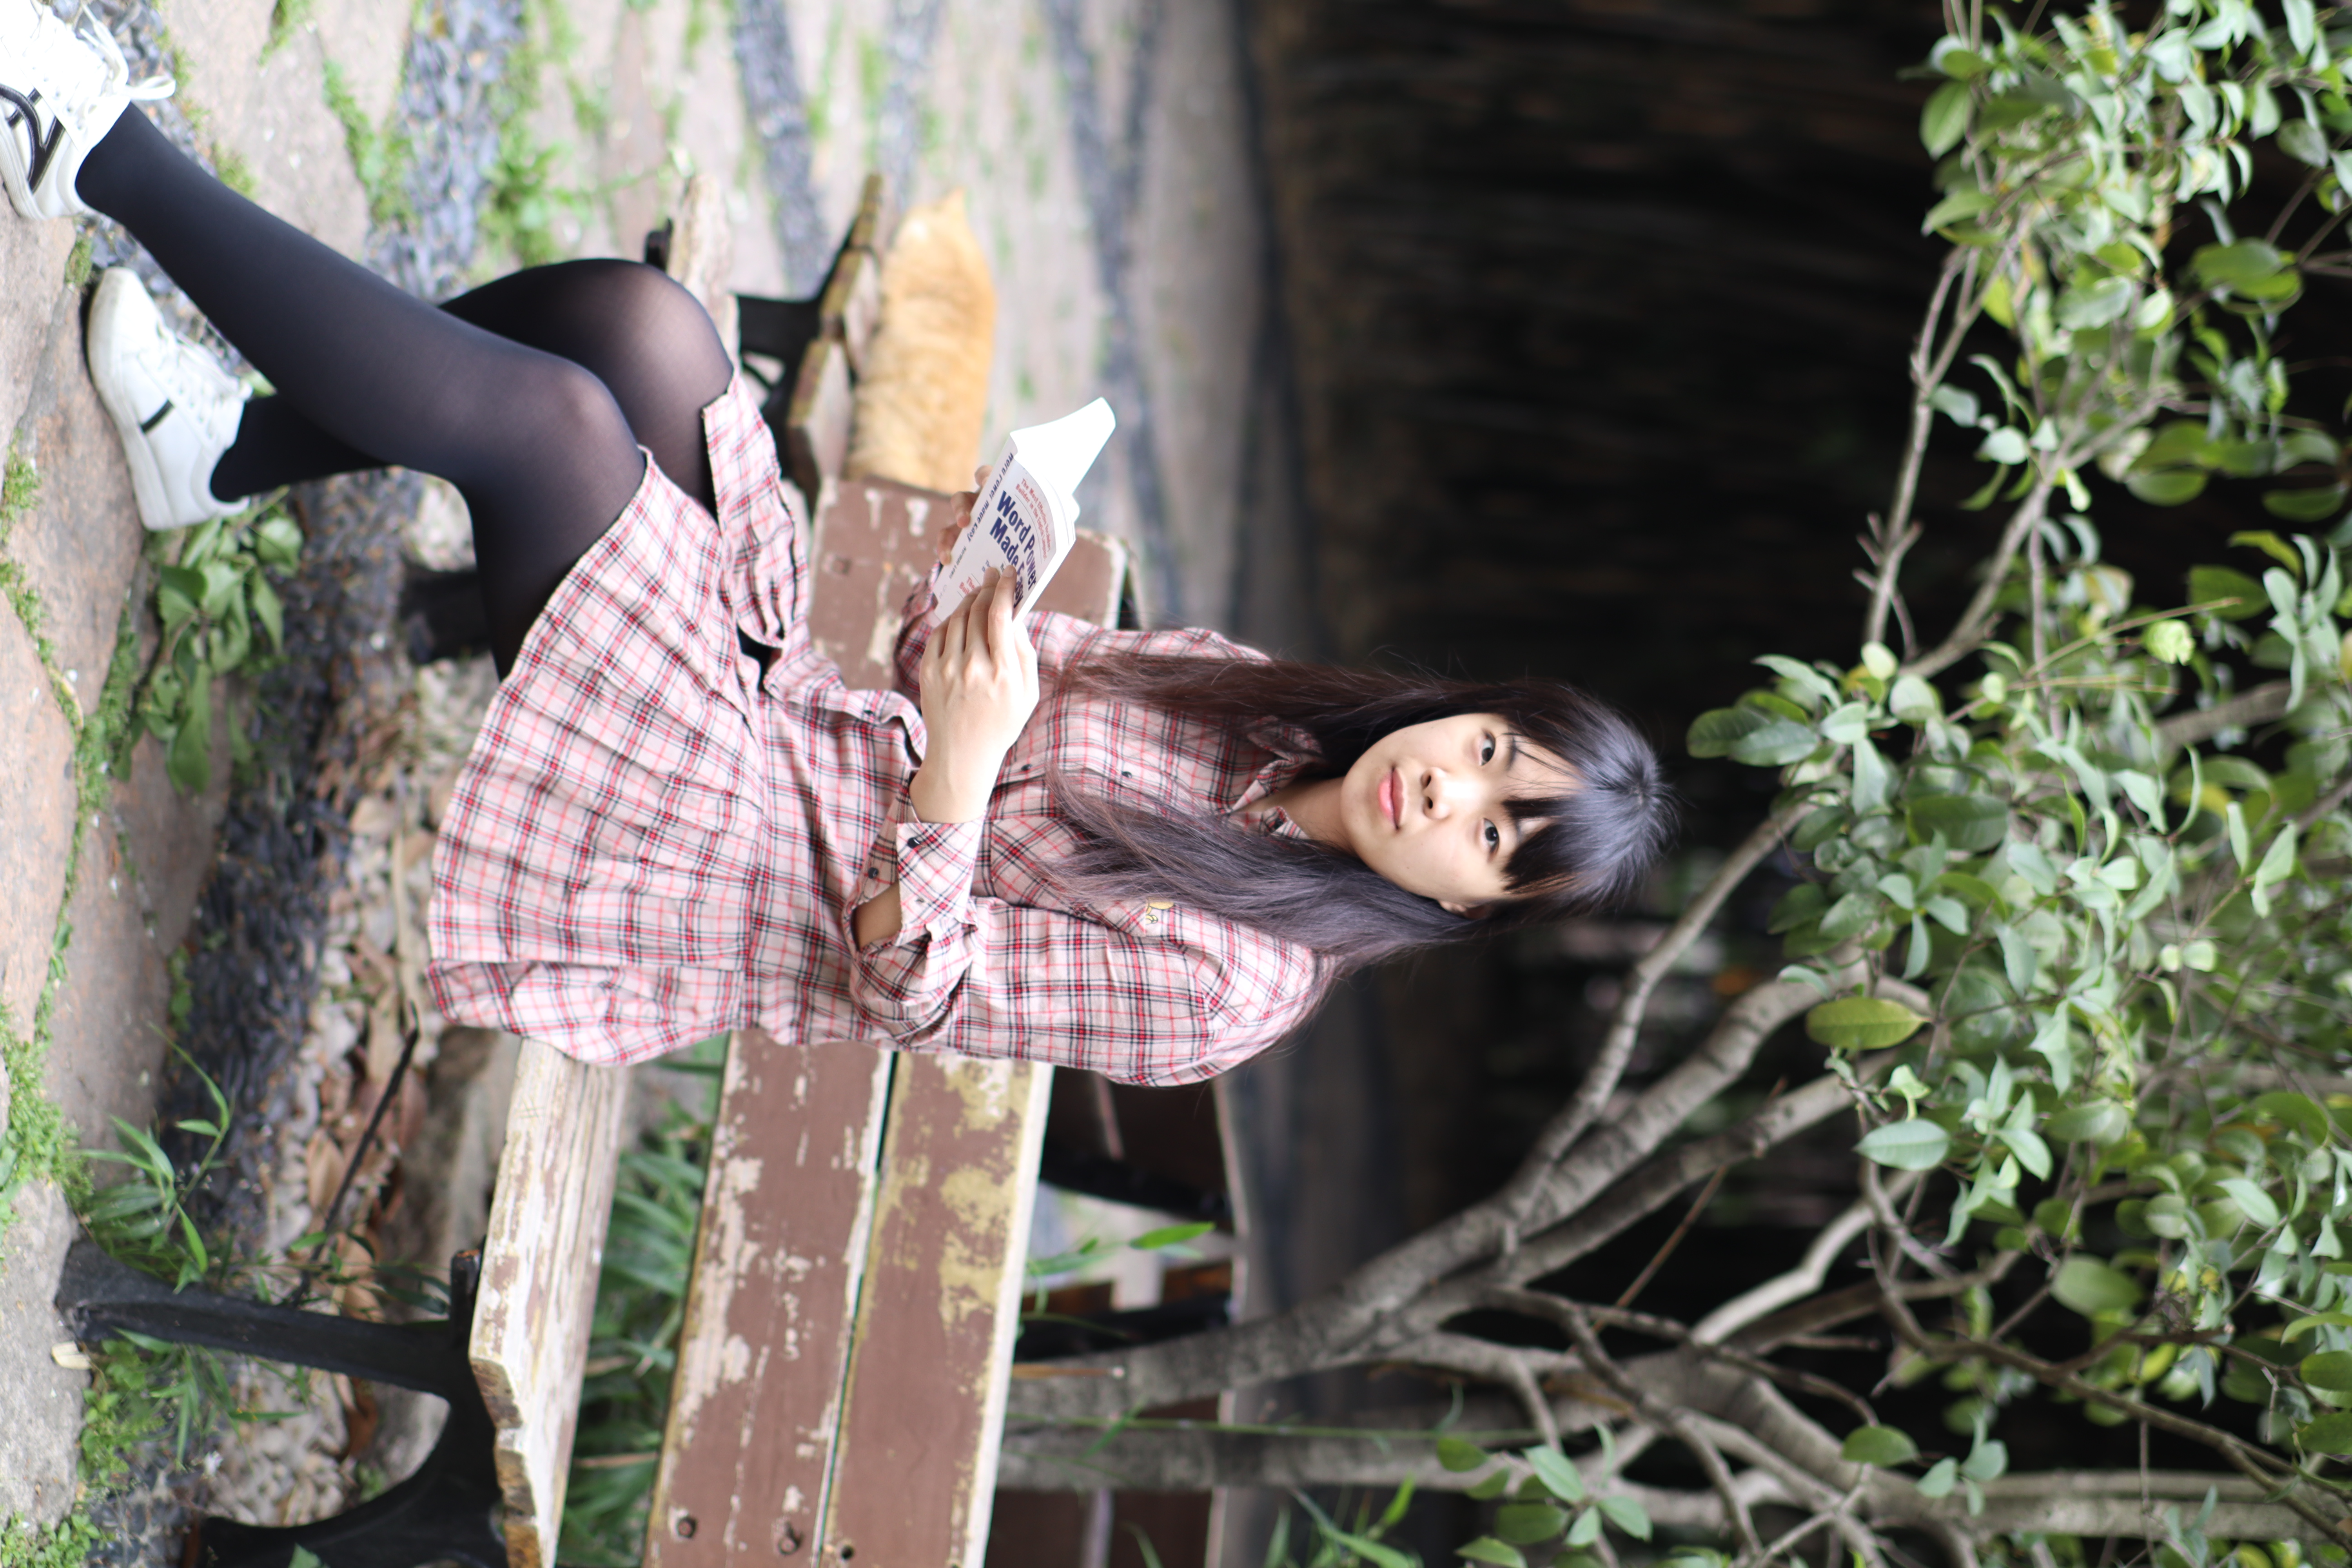
\includegraphics[width=1\textwidth]{F4}
    \caption{Alignments produced by \texttt{Water} using Gapopen/Gapextend ratio}
    \label{Fig4}
\end{figure}

\subsection{Comments}
The parameter used in \texttt{EMBOSS Needle} and \texttt{EMBOSS Water} can significantly
change the output. According to the results above, some experimental rules can be concluded.

To align homologous sequences, gap extend penalty should be set higher and global alignment is preferred, 
while if we want to determine whether the sequences have similar domains, local alignment with high penalty
on gap opening but low penalty on gap extension could be a wise choice.



\section{Please select your interested protein sequence and perform a BLAST search. First use the default parameters, then change the parameters such as word size, scoring matrix (at least three different parameters) and compare the results.}

The protein used in this section is \texttt{HBA\_HUMAN Hemoglobin subunit alpha}, retrived from \url{https://www.uniprot.org/uniprot/P69905}.

The tool used is the well-known \texttt{BLAST} \upcite{altschul_gapped_1997} (blastp), which is hosted on \url{https://blast.ncbi.nlm.nih.gov/Blast.cgi}, 
detailed parameters will be shown in the subsections below.

\subsection{Default parameters}

Using default parameters to blast (blastp) the \texttt{HBA\_HUMAN Hemoglobin subunit alpha},
the graphic summary given by the program is shown below.

\begin{figure}[H]
    \centering
    \includegraphics[width=1\textwidth]{F5}
    \caption{Blast results under Default parameters}
    \label{F5}
\end{figure}

Among the 100 results, the highest E value is $10^-91$, and the lowest identity is $95.07\%$.
Most of the results are Hemoglobin proteins from mammals, which implies that these proteins are homologous.

Next we will change one of the parameters and keep the other parameters the same to
explore how parameters will change the blast results.

\subsection{Filter and Blast results}

We exclude the results from human and the the graphic summary of blast results
\begin{figure}[H]
    \centering
    \includegraphics[width=1\textwidth]{F6}
    \caption{Blast results using a filter}
    \label{F6}
\end{figure}

As is shown above, most hits can cover nearly all of the query sequence.
Since the human is excluded from the organism, the highest E value is $10^-85$, and the lowest identity is $87.32\%$, 
which is the Hemoglobin subunit alpha \textit{Pteropus alecto} and more results from different organisms is given out by BLAST.

\subsection{Word size and Blast results}
We changed the word size and observed highest and lowest identity and E value of the results,
which is shown in the table below.

Since there is no significant change in the results in the non-redundant protein database, 
we searched in another database, the swissprot, to see whether Word size could infulence the results.

\begin{table}[H]
    \caption{Different Word size in the swissprot}
    \centering
    \begin{tabular}{ccccc}
        \toprule
        K&Best E value&Worst E value&Highest Identity&Lowest Identity\\
        \midrule
        2&$10^-101$&$10^-84$&$100\%$&$85.21\%$\\
        3&$10^-100$&$10^-84$&$100\%$&$85.21\%$\\
        6&$10^-100$&$10^-84$&$100\%$&$82.39\%$\\
        \bottomrule
    \end{tabular}
\end{table}

The slight difference in the Lowest Identity indicates that the word size can infulence search results,
but more experiments should be performed to identify the more datailed mechanism on the parameter.
However, since the ncbi hosted blast is slow due to its large number of users, large amount of queries
is almost impossible.

\subsection{Expect threshold and Blast results}
We changed the Expect threshold and observed highest and lowest identity and E value of the results,
which is shown in the table below. Other parameters are the same as above, 
but to make the impact of Expect threshold more significantly, we only include proteins in PDB.

\begin{table}[H]
    \caption{Different Expect threshold in the swissprot}
    \centering
    \begin{tabular}{ccccc}
        \toprule
        Expect threshold&Best E value&Worst E value&Highest Identity&Lowest Identity\\
        \midrule
        0.05&$10^-100$&$10^-84$&$100\%$&$44.22\%$\\
        0.50&$10^-97$&$10^-86$&$100\%$&$87.32\%$\\
        1.00&$10^-97$&$10^-86$&$100\%$&$87.32\%$\\
        \bottomrule
    \end{tabular}
\end{table}

The variance in the results is not significant, but we can still safely conclude that
the threshold can make the results more or less different.


\subsection{Scoring matrix and Blast results}

We changed the scoring matrix and observed highest and lowest identity and E value of the results,
which is shown in the table below.
Other parameters are the same as above, but to make the impact of Expect threshold more significantly, we only include proteins in PDB.


\begin{table}[H]
    \caption{Different Scoring matrix}
    \centering
    \begin{tabular}{ccccc}
        \toprule
        Scoring matrix&Max Score&Min Score\\
        \midrule
        BLOSUM62&257&98.2\\
        BLOSUM80&268&101\\
        PAM250&215&90.1\\
        PAM30&265&100\\
        \bottomrule
    \end{tabular}
\end{table}

As is shwon on the table above, for homologous sequences, BLOSOM X matrix gives out better results when X is big,
and as to PAM X matrix, when X gets smaller, the reuslts are better.

For more discussion of BLOSUM and PAM matrix, a protocol titled \textit{Comparison of the PAM and BLOSUM Amino Acid Substitution Matrices} gives more details.\upcite{mount_comparison_2008}

\subsection{A fusion protein}

To test the performance of the tool \texttt{Blast}, we constructed 
a fusion protein which has a green fluorescent protein (GFP) attached to a $\beta$-actin.

The protein sequences is listed below:
\begin{lstlisting}[frame=single]
>merged|actin-gpf
MCEEETTALVCDNGSGLCKAGFAGDDAPRAVFPSIVGRPRHQGVMVGMGQKDSYVGDEAQ
SKRGILTLKYPIEHGIITNWDDMEKIWHHSFYNELRVAPEEHPTLLTEAPLNPKANREKM
TQIMFETFNVPAMYVAIQAVLSLYASGRTTGIVLDSGDGVTHNVPIYEGYALPHAIMRLD
LAGRDLTDYLMKILTERGYSFVTTAEREIVRDIKEKLCYVALDFENEMATAASSSSLEKS
YELPDGQVITIGNERFRCPETLFQPSFIGMESAGIHETTYNSIMKCDIDIRKDLYANNVL
SGGTTMYPGIADRMQKEITALAPSTMKIKIIAPPERKYSVWIGGSILASLSTFQQMWISK
PEYDEAGPSIVHRKCFVVVVVVVVVVMSKGEELFTGVVPILVELDGDVNGHKFSVSGEGE
GDATYGKLTLKFICTTGKLPVPWPTLVTTFSYGVQCFSRYPDHMKQHDFFKSAMPEGYVQ
ERTIFFKDDGNYKTRAEVKFEGDTLVNRIELKGIDFKEDGNILGHKLEYNYNSHNVYIMA
DKQKNGIKVNFKIRHNIEDGSVQLADHYQQNTPIGDGPVLLPDNHYLSTQSALSKDPNEK
RDHMVLLEFVTAAGITHGMDELYK
\end{lstlisting}

Using blastp with default parameters to search this fusion protein, 
and the graphic summary is shwon below.

\begin{figure}[H]
    \centering
    \includegraphics[width=1\textwidth]{F7}
    \caption{Blast a fusion protein}
    \label{F7}
\end{figure}

The graphic summary clearly pointed out the two major domains of this fusion protein,
as is expected. 
This feature of BLAST can be used to identify unknown proteins with known domains, 
which is useful in the design of the experiments before we carry out them.


\section{There are some serious mistakes in his distorted analysis. Can you help him do appropriate BLAST program to get a reasonable result and make a comment?}

\textit{Dr James Lyons-Weilerc claimed SARS-CoV-2 was most likely constructed via laboratory recombination 
(https://jameslyonsweiler.com/2020/02/02/moderately-strong-confirmation-of-a-laboratory-origin-of-2019-ncov/). 
He showed SARS-CoV-2 had a unique inserted sequence (in supplement) located in the middle of its spike glycoprotein gene that had no match in other coronaviruses (Figure 1). 
Furthermore, he declared this inserted sequence was similar to some sequence in pShuttle-SN, a common expression vector used in research laboratory (Figure 2). 
Therefore, he claimed a laboratory origin of SARS-CoV-2.}

Since Dr James Lyons-Weilerc did not provide detailed parameters used in the BLAST,
we assume that he used the default parameters to do the alignment. 
Using BLAST, he found an inserted fragment in the 2019-nCoV, but not found in other bat coronaviruses, nor in SARS in the homologous genomic position, and he predicted that the inserted fragment is homologous to part of the pShuttle-SN vector.

We did a BLAST using the inserted fragment as he reported, 
and found that after excluding the results from SARS-Cov-2,
we found that the sequence can also be found in \textit{Bat coronavirus RATG13} and 
\textit{Pangolin coronavirus GX\_P4L,GX\_P5L,GX\_P5E etc}, with 99\% identity.
The sequence is also similar to a part of \textit{Bat coronavirus PrC31}, with about 80\% identity.

Considering the high mutation rate of the RNA virus, it is not reasonable to do a BLAST with default parameters,
since the default parameters are for searching very similar sequences. Although, 
the score and identity of the given sequence and some expression vector is higher than the \textit{Bat coronavirus} and \textit{Pangolin coronavirus}, more sequences form different viruses have parts that are the same as the sequence, 
which is more reasonable if we take the natural fragment recombination into consideration.

The parameters we used is to exclude SRAS-Cov2, with a smaller word size and instead of \texttt{Highly similar sequences (megablast)}, we use \texttt{More dissimilar sequences (discontiguous megablast)} and \texttt{Somewhat similar sequences (blastn)} to get more comprehensive results.

\section{Discussions}
Sequence Alignment, as some algorithms, can only produce results accoring to their input and parameters,
but they can not tell us the biology significance of the results. Before utilizing a tool, such as the BLAST or Needle,
we need to first make sure we understand how it works, what we expect to get, and how to adjust the parameters to get
the desired results.

Tools are made for man, when man should not be slave of a tool.


\section{Supplementary materials}

\subsection{A typical output of \texttt{Needle} and \texttt{Water} alignment}

\begin{lstlisting}[frame=single]
########################################
# Program: needle
# Rundate: Sat 17 Apr 2021 16:52:56
# Commandline: needle
#    -auto
#    -stdout
#    -asequence emboss_needle-I20210417-165603-0006-72965156-p1m.asequence
#    -bsequence emboss_needle-I20210417-165603-0006-72965156-p1m.bsequence
#    -datafile EBLOSUM80
#    -gapopen 10.0
#    -gapextend 0.5
#    -endopen 10.0
#    -endextend 0.5
#    -aformat3 pair
#    -sprotein1
#    -sprotein2
# Align_format: pair
# Report_file: stdout
########################################

#=======================================
#
# Aligned_sequences: 2
# 1: HBA_HUMAN
# 2: HBA_MOUSE
# Matrix: EBLOSUM80
# Gap_penalty: 10.0
# Extend_penalty: 0.5
#
# Length: 142
# Identity:     122/142 (85.9%)
# Similarity:   131/142 (92.3%)
# Gaps:           0/142 ( 0.0%)
# Score: 1043.0
# 
#
#=======================================

HBA_HUMAN          1 MVLSPADKTNVKAAWGKVGAHAGEYGAEALERMFLSFPTTKTYFPHFDLS     50
                     ||||..||:|:||||||:|.|..|||||||||||.|||||||||||||:|
HBA_MOUSE          1 MVLSGEDKSNIKAAWGKIGGHGAEYGAEALERMFASFPTTKTYFPHFDVS     50

HBA_HUMAN         51 HGSAQVKGHGKKVADALTNAVAHVDDMPNALSALSDLHAHKLRVDPVNFK    100
                     |||||||||||||||||.:|..|:||:|.|||||||||||||||||||||
HBA_MOUSE         51 HGSAQVKGHGKKVADALASAAGHLDDLPGALSALSDLHAHKLRVDPVNFK    100

HBA_HUMAN        101 LLSHCLLVTLAAHLPAEFTPAVHASLDKFLASVSTVLTSKYR    142
                     |||||||||||:|.||:|||||||||||||||||||||||||
HBA_MOUSE        101 LLSHCLLVTLASHHPADFTPAVHASLDKFLASVSTVLTSKYR    142


#---------------------------------------
#---------------------------------------
\end{lstlisting}

\bibstyle{unsrt}
\bibliography{references}{}
\end{document}
